\documentclass[review]{elsarticle}

\usepackage{lineno,hyperref}
\usepackage{wasysym}
\usepackage{pgfplots}
\usepgfplotslibrary{dateplot, statistics}
\usepackage{titlesec}
\setcounter{secnumdepth}{3}
\titleformat{\paragraph}
{\normalfont\normalsize\bfseries}{\theparagraph}{1em}{}
\titlespacing*{\paragraph}
{0pt}{3.25ex plus 1ex minus .2ex}{1.5ex plus .2ex}

\modulolinenumbers[5]

\journal{Journal of \LaTeX\ Templates}


%% This is where all the data go (temp)
\pgfplotstableread[row sep=\\,col sep=&]{
    location & number \\
    Club Field & 5 \\
    Headmaster's Field & 2 \\
    South Field & 5 \\
    Boardwalk & 5 \\
}\locationpick 

\pgfplotstableread[row sep=\\,col sep=&]{
    location & yes & no \\
    Club Field & 7 & 5\\
    South Field & 1 & 11\\
    Boardwalk & 4 & 8\\
}\locationbeauty

\pgfplotstableread[col sep=comma]{../Data/1day/windata10m.csv}\windonedaytenminutes
\pgfplotstableread[col sep=comma]{../Data/1day/windata1hr.csv}\windonedayonehour

\pgfplotstableread[col sep=comma]{../Data/1week/windata30m.csv}\windoneweekthirtyminutes
\pgfplotstableread[col sep=comma]{../Data/1week/windata4hr.csv}\windoneweekfourhour

\pgfplotstableread[col sep=comma]{../Data/1month/windata2h.csv}\windonemonthtwohour
\pgfplotstableread[col sep=comma]{../Data/1month/windata12h.csv}\windonemonthtwelvehour
\pgfplotstableread[col sep=comma]{../Data/1month/windata1d.csv}\windonemonthoneday
%%%%%%%%%%%%%%%%%%%%%%%%%%%%%%%%%%%%%%%%

%%%%%%%%%%%%%%%%%%%%%%%
%% Elsevier bibliography styles
%%%%%%%%%%%%%%%%%%%%%%%
%% To change the style, put a % in front of the second line of the current style and
%% remove the % from the second line of the style you would like to use.
%%%%%%%%%%%%%%%%%%%%%%%

%% Numbered
%\bibliographystyle{model1-num-names}

%% Numbered without titles
%\bibliographystyle{model1a-num-names}

%% Harvard
%\bibliographystyle{model2-names.bst}\biboptions{authoryear}

%% Vancouver numbered
%\usepackage{numcompress}\bibliographystyle{model3-num-names}

%% Vancouver name/year
%\usepackage{numcompress}\bibliographystyle{model4-names}\biboptions{authoryear}

%% APA style
\bibliographystyle{model5-names}\biboptions{authoryear}

%% AMA style
%\usepackage{numcompress}\bibliographystyle{model6-num-names}

%% `Elsevier LaTeX' style
%\bibliographystyle{elsarticle-num}

%%%%%%%%%%%%%%%%%%%%%%%

\begin{document}
\begin{frontmatter}

\title{The Feasibility of Small-Scale Wind Power Generation at Kent School, Connecticut: \\An economic, environmental, and aesthetic analyses}

%% Group authors per affiliation:
\author{Jiajun Mao, Chun Lam Cheng}
\address{1 Macedonia Rd., Kent, CT}
\fntext[myfootnote]{Since 1880.}

\begin{abstract}
\indent Carbon-based energy source in electricity generation has already been challenged, in multiple researches, not only for their scarcity(\cite{mikael_depletion_of_fossil_fuel}) 
but also their negative impacts on earth’s environment. In face of severe environmental challenges such as global warming and its resulting problems such as extreme 
weathers(\cite{mikael_depletion_of_fossil_fuel}) and dramatically increasing species, such as amphibian's, extinction rate(\cite{alan_amphibian_extinction}), a clean and 
environmentally-friendly energy source is in need. It is evidence through multiple researches that wind power has the potential of subsidizing, if not replacing, the role of 
power generation by those traditional energy sources. In light of the development of wind power worldwide, it is important for Kent School to also consider using wind power to 
fulfill parts of the electricity consumption on campus and hopefully reduce campus’ environmental footprint. This study specifically focuses on the feasibility of a small-scale 
wind farm on Kent School’s campus through economic, environmental and aesthetic perspectives.
\end{abstract}

\begin{keyword}
Wind \sep Kent School\sep Small-scale \sep Energy \sep Economic-feasibility
\end{keyword}

\end{frontmatter}

\linenumbers

\clearpage
\section{Introduction}
\label{sec:Introduction}

Kent School receives its electricity from the CT state grid [CONFIRM] (the solar power generated is sold back to the power company), which means that according to the 
energy sources profile of the CT state grid, 63.7\% of the electricity that Kent School uses comes from natural gas and 31.2\% comes from nuclear. Also, the data obtained 
from Kent School’s Maintenance Department shows that the annual power consumption is [CONFIRM] MWh. Calculating from the average commercial electricity rates in the state 
of Connecticut, which is 14.65 cents/kWh, the annual spending of Kent School on electricity consumption is roughly [CONFIRM]. Therefore, the incentives for the installation 
of wind power generation facility on campus can be concluded into two following parts:
\begin{itemize}
    \item \textit{\textbf{environmental incentives.}} Reduction of school's overall environmental footprint in hope of contriubting to the alleviation of environmental 
    problems caused by electricity consumption worldwide.
    \item \textit{\textbf{economic incentives.}} Reduction of school's growing expenditure incurred by student's growing demand in electricity so that school can reach 
    tuition/expenditure balance with each student.
\end{itemize}

\subsection{environmental incentives}
\label{sec:intro:environincentives}
Though natural gas is a comparably cleaner energy source than traditional carbon-based sources such as coal or petroleum, the burning of natural gas nevertheless still 
releases carbon dioxide (\cite{cost_and_performance_baseline_for_fossil_energy_plants}), one of the most notorious greenhouse gases that are causing the global 
warming(\cite{Shakun2012_co2_global_warming}). Therefore, for environmental concerns, the burning of carbon-based energy source should be avoided as much as possible. 
Wind power, despite the carbon emission generated during the manufacturing processes of the turbines (\cite{Kaldellis_carbon_foortprint_of_offshore_wind_energy}), release 
mininum, if not none, additional green house gases once they become functional (\cite{IEEE_wind_carbon_reduction}).
\\\indent Several reviews have been done regarding the potential or achievement of wind power in reducing the overall carbon emission and other environmentally harmful 
gas for electricity generation, as well as our reliance on fossil fuels. These studies, including \cite{rajat_cost_saving_and_emission_reduction}'s Cost savings and 
emission reduction capability of wind-integrated power systems and \cite{IEEE_wind_carbon_reduction}'s Wind Generation, Power System Operation, and Emission Reduction 
demonstrate the possibility and potential of reduction in Kent School’s carbon footprint if wind-power generating facilities are installed on campus, which will in turn 
further Kent’s path on making the school’s operations more environmentally sustainable.
 

\subsection{economic incentives}
\label{sec:intro:econincentives}
It is evident that to provide students with quality education, Kent School needs to possess certain degree of financial affluency. However, according to various sources, 
including the Headmaster of the school, Fr. Shell, and the annual report of Kent School [NEED], there is a substantial gap existing between the tuition and cost for a 
student. Therefore, to make Kent education truly available to everyone, the operational cost gap for each student must be reduced. Using wind energy to subsidize the 
electricity consumption on campus might make the cost reduction possible.
\\\indent Again, several studies, including Maria Isabel Blanco’s The economics of wind energy (\cite{maria_wind_energy_economics}), and The Economics of Wind Energy: 
A report by the European Wind Energy Association (\cite{european_wind_energy_association_report}), prove that the average cost of operating wind farm could be substantially 
lower compared to the cost of buying electricity from the regional power. Therefore, through the utilization of wind power on campus, Kent School can possibility reduce the 
operation cost for a single student become more financially self-sufficient, in turn providing future Kent students a better education.   


\section{Methods}
\label{sec:methods}

\subsection{Location Determination Factors}
When determining the location of the possible wind farm, the location must satisfy the requirements including but not limited to the listed below. When considering a 
location, requirement 1 and 2 are strict requirement, meaning that if these two requirements are not fulfilled, a location should not be considered even if they satisfy 
requirement 3 and 4.
Requirement 3 and 4 in turn, are loose requirements that do not necessarily have to be fulfilled if economic and environmental benefit of constructing a wind farm outweight 
the negative influence. However, if there is a statistically significant portion of student body voicing against the constructin of the wind farm for the reason mentioned 
in requirement 3 and 4, 
these two requirements will be weighted more heavily into consideration of the location of the wind farm.

\begin{enumerate}
    \item \emph{Power and consistent wind.} Whether that location has consistent and powerful wind to make the construction of a wind farm viable. The rough wind speed 
    of that location is reported by students on campus and Jiajun and Chu Lam's personal experience around the campus.
    \item \emph{Feasible location.} Whether that location has enough space on the ground and in the air to support the construction of a wind farm. This factor is determined 
    by the proximity to another physical object on the ground level or in the air, such as dormitories, academic/religious buildings, mountains, etc.
    \item \emph{Minimal influence on school operations.} Whether the prescence of a wind farm at that location will cause disturbance or negative influence on normal daily 
    school operations. For example, the noise generated by the wind turbine is factored into considerations.
    \item \emph{Minimal influence on aesthetic beauty.} Whether the construction of a wind farm at that location will decrease the beauty of the lovely valley land of Kent. 
    This factor is majorly based on Jiajun and Chu Lam's subjectie defintion of beauty.
\end{enumerate}

\subsection{Location Determination Process}
\label{sec:methods:locdeterprocess}
In order to obtain a general location on campus where the wind is consistent and powerful, a study is done with students population on campus. By assigning each of CL and 
Jiajun's 54 friends a number and by using a random number generator, we were able to select 30 students to respond to the question of 
\textit{"Where on campus do you think the wind is strongest? And another location where the wind is the second strong?"}. From the all the responses we receive, we will 
determine two location with the highest vote and consider them for the second requirement of location feasibility. Taking the second requirement into consideration - location feasibility, 
we will analyze both sites' proximity to another physical object and conclude whether the two 
 sites from the requirement above satisfy the criteria of having a clear ground level and aerial zone for the construction of a possible wind farm. If any location does 
 not satisfy the criteria for this requirement, it will be eliminated from consideration. Then, from the remaining locations we will analyze their potential influence 
 on school's normal operation, including but not limited to academic activities, atheletic activities, and recreational activities. The negative effects of wind farm will 
 be analyzed and considered such as the noise generated and the space required on the ground level. At last, the remaining sites might cause influence on the aesthetic beauty 
 of the Housatonic valley. A study identical to the one described in requirement one is conducted again with the question \textit{"Do you think the construction of a wind 
 farm at site A and/or B will have negative impact on the aesthetic beauty of the surrouding area and the Kent campus?"} From the answers received we will analyze the 
 majority side and take that into consideration. 

\subsection{Feasibility Determination Process}
\label{sec:methods:feasdeterprocess}
After the location is determined by the process described in section 2.2, they will be analyzed for the feasbility of actually constructing a wind farm. Relevant data 
such as flow volume and wind speed will be collected. To collect such data, HoldPeak's wind anemometer 856A will be used. The device will be setup in the chosen location 
and the fan that will be measuring the wind speedwill be setup on top of a tripod 2m above ground level. After a continuous 24 hours of data collection, the data from the 
wind anemometer is then transferred to the computer and a graph of wind speed/flow volume against time will be plotted.
\\\indent From the plotted graph as well as the wind speed/flow volume's relationship with the amount of electricity generateed we can estimate the economic benefit from 
the construction of such a wind farm and its possible environmental benefits and consequences. At last we can compare the wind speed and flow volume, as well as the 
economic/environmental benefit of different locations across campus with each other and other locations in the United States where commercial wind farms are in operation 
to determine the final feasibility of constructing a wind farm on Kent School's property at a chosen location.



\section{Results}
\label{sec:results}
\subsection{Location Determination Results}
\label{sec:results:locdeterresults}
After sending out requests to 60 students on campus with the question \textit{Where do you think the wind is strongest on campus?} and the options as following,
\begin{enumerate}
    \item {Club Field}
    \item {Headmaster's Field}
    \item {South Field}
    \item {Boardwalk/Main}   
\end{enumerate}
we received 17 response from those 60 questionnaires sent, a response rate of 28.3\%. The result of the survey is demonstrated in \textit{Figure \ref{fig:locationpick}} with Club Field, South Field, and Boardwalk each receiving 5 votes and Headmaster's Field Receiving 2. 
%TODO: Change the question in the methods section to make sure the paper is not self-conflicting

\clearpage

\begin{figure}
    \caption{Location of Strongest Wind at Kent School}
    \begin{tikzpicture}
        \begin{axis}[
                ybar,
                bar width=1.2cm,
                width = \textwidth,
                height = 0.4*\textwidth,
                symbolic x coords={Club Field,Headmaster's Field,South Field,Boardwalk},
                xtick=data,
                nodes near coords,
                ylabel={Numbers of Responses},
                ymax=7,
                ymin=0,
            ]
            \addplot table[x=location,y=number]{\locationpick};
        \end{axis}
    \end{tikzpicture}
    \label{fig:locationpick}
\end{figure}

From the 60 survey we sent out to random Kent students with the question \textit{Will Installing Wind Turbines at Following Locations Disrupt the Beautiful Kent Scneary} 
and the following choices,
\begin{enumerate}
    \item Club Field
    \item South Field
    \item Boardwalk/Main
\end{enumerate}

we received 12 responses from those 60 questionnaires, a resposne rate of 20\%. The result of the survey is demonstrated in \textit{Figure \ref{graph:locationbeauty}} with 58\% of responses saying yes 
for Club Field, 8.3\% of responses saying yes to South Field, and 33.4\% of responses saying yes to Boardwalk.\\

\begin{figure}[!h]
    \caption{Will Installing Wind Turbines Disrupt Kent Scenery?}
    \begin{tikzpicture}
        \begin{axis}[
                ybar,
                enlarge x limits = {abs=1.8cm},
                legend style={                    
                legend cell align=right,       
                legend columns=1,    
                anchor=west}, 
                area legend,
                bar width=1.2cm,
                width = \textwidth,
                height = 0.4*\textwidth,
                symbolic x coords={Club Field,South Field,Boardwalk},
                xtick=data,
                nodes near coords,
                ylabel={Numbers of Responses},
                ymax=13,
                ymin=0,
            ]
            \addplot table[x=location,y=yes]{\locationbeauty};
            \addplot table[x=location,y=no]{\locationbeauty};
            \addlegendentry{yes}
            \addlegendentry{no}
        \end{axis}
        \label{graph:locationbeauty}
    \end{tikzpicture}
\end{figure}

\clearpage
\subsection{Location Wind Speed Result}
\label{sec:results:locwindspeedresults}
For reasons mentioned \textit{\ref{sec:analysis:erroranalysis:datadestruction}}  of the error analysis, only wind speed data from the anemometer on top of Dickinson Auditorium is preserved and recorded. We have manged to obtain 
the wind data for a single day (5/22/2019), an entire week (5/15-5/22/2019) and an entire month (4/22-5/22/2019). For each individual time period we plotted the detail wind speed data 
averaged for relatively small time frame to accurately reflect the wind speed during that period of time while preserving the visibility in the graphed plots. Then for each time frame 
we plotted an extra graph using a moving average of a longer period of time, which shows the general trend of the wind speed.
\\\indent It can be seen from \textit{Figure \ref{wind:oneday:onehour}}(single day) that for a single day during spring time, highest wind speed occurs during midday with wind speed reaching as high as 2m/s while the wind 
speed during morning and evening are only around 0.5m/s. It can also be seen from \textit{Figure \ref{wind:oneweek:fourhour}}(entire week) that the general trend of wind speed during a week corresponds to daily trend without 
a clear weekly trend. At last, we can see from \textit{Figure \ref{wind:onemonth:oneday}} that wind speed is generally higher at the end of a month.

%TODO: might change after more data is added to the plot

\vspace{100pt}
\textit{\textbf{Graphs are on next page for better formatting}}

\clearpage

%%%%%%%%%%%%%%%%%%%%%%%%%%%%%%%%%%%%%%%%%%%%%%%%%%%%%%%
% One Day%
%%%%%%%%%%%%%%%%%%%%%%%%%%%%%%%%%%%%%%%%%%%%%%%%%%%%%%%

\begin{figure}
    \caption{Wind Speed(Boardwalk) on 5/22/2019 Averaged for 10m}
    \begin{tikzpicture}
        \begin{axis}[
            xlabel=time,
            x label style={at={(axis description cs:1.05,0.12)},anchor=north},
            ylabel=Wind Speed(m/s), 
            date coordinates in=x, 
            table/col sep=comma, 
            date ZERO=2019-05-22, 
            xticklabel=\month.\day. \hour:\minute, 
            width=\textwidth,
            height=0.54\textwidth,
            xticklabel style={rotate=90, anchor=near xticklabel},
            title style={anchor=north,yshift=20}
            ]
            \addplot+[no markers] table[x=Time,y=WS (m/s)] {\windonedaytenminutes};
        \end{axis}
    \end{tikzpicture}
    \label{wind:oneday:tenminutes}
\end{figure}

\vspace{40pt}

\begin{figure}
    \caption{Wind Speed(Boardwalk) on 5/22/2019 Averaged for 1hr}
    \begin{tikzpicture}
        \begin{axis}[
            xlabel=time,
            x label style={at={(axis description cs:1.05,0.12)},anchor=north},
            ylabel=Wind Speed(m/s), 
            date coordinates in=x, 
            table/col sep=comma, 
            date ZERO=2019-05-22, 
            xticklabel=\month.\day. \hour:\minute,
            width=\textwidth,
            height=0.54\textwidth,
            xticklabel style={rotate=90, anchor=near xticklabel},
            ]
            \addplot+[no markers] table[x=Time,y=WS (m/s)] {\windonedayonehour};
        \end{axis}
    \end{tikzpicture}
    \label{wind:oneday:onehour}
\end{figure}

%%%%%%%%%%%%%%%%%%%%%%%%%%%%%%%%%%%%%%%%%%%%%%%%%%%%%%%
%One Week%
%%%%%%%%%%%%%%%%%%%%%%%%%%%%%%%%%%%%%%%%%%%%%%%%%%%%%%%

\begin{figure}
    \caption{Wind Speed(Boardwalk) 5/15-5/22/2019 Averaged for 30m}
    \begin{tikzpicture}
        \begin{axis}[
            xlabel=time, 
            x label style={at={(axis description cs:1.05,0.12)},anchor=north},
            ylabel=Wind Speed(m/s), 
            date coordinates in=x, 
            table/col sep=comma, 
            date ZERO=2019-05-17, 
            xticklabel=\month.\day. \hour:\minute, 
            width=\textwidth,
            height=0.54\textwidth,
            xticklabel style={rotate=90, anchor=near xticklabel},
            ]
            \addplot+[no markers] table[x=Time,y=WS (m/s)] {\windoneweekthirtyminutes};
        \end{axis}
    \end{tikzpicture}
    \label{wind:oneweek:thirtyminutes}
\end{figure}

\vspace{40pt}

\begin{figure}
    \caption{Wind Speed(Boardwalk) 5/15-5/22/2019 Averaged for 4hr}
    \begin{tikzpicture}
        \begin{axis}[
            xlabel=time, 
            x label style={at={(axis description cs:1.05,0.12)},anchor=north},
            ylabel=Wind Speed(m/s), 
            date coordinates in=x, 
            table/col sep=comma, 
            date ZERO=2019-05-17, 
            xticklabel=\month.\day. \hour:\minute, 
            width=\textwidth,
            height=0.54\textwidth,
            xticklabel style={rotate=90, anchor=near xticklabel},
            ]
            \addplot+[no markers] table[x=Time,y=WS (m/s)] {\windoneweekfourhour};
        \end{axis}
    \end{tikzpicture}
    \label{wind:oneweek:fourhour}
\end{figure}

%%%%%%%%%%%%%%%%%%%%%%%%%%%%%%%%%%%%%%%%%%%%%%%%%%%%%%%
%One Month%
%%%%%%%%%%%%%%%%%%%%%%%%%%%%%%%%%%%%%%%%%%%%%%%%%%%%%%%

\begin{figure}
    \caption{Wind Speed(Boardwalk) 4/22-5/22/2019 Averaged for 2hr}
    \begin{tikzpicture}
        \begin{axis}[
            xlabel=time,
            x label style={at={(axis description cs:1.05,0.12)},anchor=north},
            ylabel=Wind Speed(m/s), 
            date coordinates in=x, 
            table/col sep=comma, 
            date ZERO=2019-04-22, 
            xticklabel=\month.\day. \hour:\minute, 
            width=\textwidth,
            height=0.54\textwidth,
            xticklabel style={rotate=90, anchor=near xticklabel},
            ]
            \addplot+[no markers] table[x=Time,y=WS (m/s)] {\windonemonthtwohour};
        \end{axis}
    \end{tikzpicture}
    \label{wind:onemonth:twohour}
\end{figure}

\vspace{40pt}

\begin{figure}
    \caption{Wind Speed(Boardwalk) 4/22-5/22/2019 Averaged for 1 day}
    \begin{tikzpicture}
        \begin{axis}[
            xlabel=time, 
            x label style={at={(axis description cs:1.05,0.12)},anchor=north},
            ylabel=Wind Speed(m/s), 
            date coordinates in=x, 
            table/col sep=comma, 
            date ZERO=2019-04-22, 
            xticklabel=\month.\day. \hour:\minute, 
            width=\textwidth,
            height=0.54\textwidth,
            xticklabel style={rotate=90, anchor=near xticklabel},
            ]
            \addplot+[no markers] table[x=Time,y=WS (m/s)] {\windonemonthoneday};
        \end{axis}
    \end{tikzpicture}
    \label{wind:onemonth:oneday}
\end{figure}

%%%%%%%%%%%%%%%%%%%%%%%%%%%%%%%%%%%%%%%%%%%%%%%%%%%%%%%
%%%%%%%%%%%%%%%%%%%%%%%%%%%%%%%%%%%%%%%%%%%%%%%%%%%%%%%

\clearpage
\subsection{Location Power Output Result}
\label{sec:results:locationpowerresults}

%%%%%%%%%%%%%%%%%%%%%%%%%%%%%%%%%%%%%%%%%%%%%%%%%%%%%%%
% One Day%
%%%%%%%%%%%%%%%%%%%%%%%%%%%%%%%%%%%%%%%%%%%%%%%%%%%%%%%

\begin{figure}[!h]
    \caption{Instantaneous Power Generation(Boardwalk) on 5/22/2019 Averaged for 10m}
    \begin{tikzpicture}
        \begin{axis}[
            xlabel=time,
            x label style={at={(axis description cs:1.05,0.12)},anchor=north},
            ylabel=Power (kW), 
            date coordinates in=x, 
            table/col sep=comma, 
            date ZERO=2019-05-22, 
            xticklabel=\month.\day. \hour:\minute, 
            width=\textwidth,
            height=0.54\textwidth,
            xticklabel style={rotate=90, anchor=near xticklabel},
            title style={anchor=north,yshift=20}
            ]
            \addplot+[no markers] table[x=Time,y=Power (kw)] {\windonedaytenminutes};
        \end{axis}
    \end{tikzpicture}
    \label{power:oneday:tenminutes}
\end{figure}

%%%%%%%%%%%%%%%%%%%%%%%%%%%%%%%%%%%%%%%%%%%%%%%%%%%%%%%
%One Week%
%%%%%%%%%%%%%%%%%%%%%%%%%%%%%%%%%%%%%%%%%%%%%%%%%%%%%%%

\begin{figure}[!h]
    \caption{Instantaneous Power Generation((Boardwalk) 5/15-5/22/2019 Averaged for 30m}
    \begin{tikzpicture}
        \begin{axis}[
            xlabel=time, 
            x label style={at={(axis description cs:1.05,0.12)},anchor=north},
            ylabel=Power (kW), 
            date coordinates in=x, 
            table/col sep=comma, 
            date ZERO=2019-05-17, 
            xticklabel=\month.\day. \hour:\minute, 
            width=\textwidth,
            height=0.54\textwidth,
            xticklabel style={rotate=90, anchor=near xticklabel},
            ]
            \addplot+[no markers] table[x=Time,y=Power (kw)] {\windoneweekthirtyminutes};
        \end{axis}
    \end{tikzpicture}
    \label{power:oneweek:thirtyminutes}
\end{figure}

%%%%%%%%%%%%%%%%%%%%%%%%%%%%%%%%%%%%%%%%%%%%%%%%%%%%%%%
%One Month%
%%%%%%%%%%%%%%%%%%%%%%%%%%%%%%%%%%%%%%%%%%%%%%%%%%%%%%%

\begin{figure}[!h]
    \caption{Instantaneous Power Generation((Boa    brdwalk) 4/22-5/22/2019 Averaged for 2hr}
    \begin{tikzpicture}
        \begin{axis}[
            xlabel=time,
            x label style={at={(axis description cs:1.05,0.12)},anchor=north},
            ylabel=Power (kW), 
            date coordinates in=x, 
            table/col sep=comma, 
            date ZERO=2019-04-22, 
            xticklabel=\month.\day. \hour:\minute, 
            width=\textwidth,
            height=0.54\textwidth,
            xticklabel style={rotate=90, anchor=near xticklabel},
            ]
            \addplot+[no markers] table[x=Time,y=Power (kw)] {\windonemonthtwohour};
        \end{axis}
    \end{tikzpicture}
    \label{power:onemonth:twohour}
\end{figure}

%%%%%%%%%%%%%%%%%%%%%%%%%%%%%%%%%%%%%%%%%%%%%%%%%%%%%%%
%%%%%%%%%%%%%%%%%%%%%%%%%%%%%%%%%%%%%%%%%%%%%%%%%%%%%%%


\section{Analysis}
\label{sec:analysis}

\subsection{Location Determination Analysis}

Combining the result shown in \textit{Figure \ref{fig:locationpick}} the processses described in \textit{Section \ref{sec:methods:locdeterprocess}}, Club Field, South Field and 
Boardwalk all satisfy the the Location Determination Factor 1 (powerful and consistent wind) from the survey result and thus qualify for being considered for the Location Determination Factor 2 (feasible location).  %/TODO: Conduct statisitcal test
\\\indent Both South Field and Club Field do not have any buildings or natural landscape such as Mount Algos in proximity, therefore they have a clear ground level that would 
be suitable for the construction of wind farm. We can also see that both South Field and Club Field satify the entirty of the Location Determination Factor 2 by not only having 
a clear ground level but a clear air space above. On the other hand, boardwalk/main is in close proximity to Dickinson Auditorium, Foley Hall and North Dorm, which makes it an 
impossible location to construct a wind farm due to unclear ground level, thus removed from consideration. As the result, only South Field and Club Field qualify for being 
considered for Location Determination Factor 3 (minimal influence on school operations).
\\\indent South Field and Club Field are fields activitely used for majority of outdoor atheletic trainings and events during the fall and spring terms of Kent School. Hence, 
having a wind farm at those two locations might have impacts on school operations during the construction phase, operation phase, and decommission phase. During the construction 
phase, areas on both of the fields will be appropriated for the construction of roads for transportation of building materials and passage of construction vehicles, as well as
temporary placement of building materials. Therefore, no atheletic events and trainings can be carried out during the construction phase. After the construction ended and the wind 
turbines are in operation, both fields still need to go through recovery period for all the grass that is necessary for atheletic events and trainings to grow back. Therefore, we 
can predict that atheletic programs of Kent School are going to be severely disrupted if the construction happens during an academic school year. A solution does exist for the school 
to construct the wind farm during summer session, which gives Kent School 3 months to finish construction. However, if the construction does not finish in that time frame, disturbances 
to school operations described above are still going to happen. %TODO: Cite construction period of a wind farm

Because 91.7\% of the people responded think that constructing a wind farm at South Field would not disrupt the landscape of Kent School, South Field satifies Location Determination Factor 4 
and qualify to become one of the potential site for the construction of the wind farm. Surprisingly, though being an open field similar to South Field, 58\% of people responded think that constructing
a wind farm at Club Field would actually disrupt the beautiful landscape of Kent School. This might be caused by Club Field's close proximity to the main campus so that students will be able to 
have the wind farm in visual at a higher frequency whereas students rarely visit South Field other than atheletic trainings and events and South Field is relatively far away from the main campus. 
However, since 58\% is not statistically significantly higher than 50\%, we cannot arrive at the conclusion that majority of the Kent Students will think that constructing a wind farm at Club Field 
will have negative impacts on the Kent landscape. As the result, Club Field will also be considered as a qualifying location for building a wind farm.
\\\indent To our surprise, only 33.4\% of people responded think that having a wind farm at Boardwalk is going to have negative impacts on Kent scenery considering the location of the Boardwalk - at the center of 
the main campus and in close proximity to areas of frequency academic activities and student life (dormitories, dining hall, chapel, etc.). Therefore, because of the reason mentioned in \textit{Section \ref{sec:analysis:erroranalysis:datadestruction}} of 
error analysis, we kept Boardwalk/main for the feasibility analysis despite the fact that it does not satisfy Location Determination Factor 2, which is a strict requirement.
\\\indent To conclude, Club Field, South Field and Boardwalk/Main all will be considered as qualifying locations for the construction of a wind farm for Kent School and all threee locations will be analyzed 
for their wind speed to determine whether the economic and environmental benefits of building a wind farm at that location will outweigh the environmental cost and disturbances to the school operation.
%TODO: a statistical test


\subsection{Feasibility Analysis}

Because of the reason mentioned \textit{Section \ref{sec:analysis:erroranalysis:datadestruction}}, we only have the data available from the AQM65 on top of Dickinson Auditorium and a selection of its data is plotted 
from \textit{Figure \ref{wind:oneday:tenminutes}} to \textit{\ref{wind:onemonth:oneday}}. Since we lack of data regarding wind speed at South Field and Club Field, we cannot determine the feasibility of constructing a 
wind farm at that location. Therefore, we are only able to determine whether it is feasible to construct a wind farm somewhere near Boardwalk with the data obtained. A wind turbine's power output can 
be calculated with the following equation:
\begin{equation}
    \label{equ:windpower}
    P=1/2*k*C_{p}*\rho*A*V^3
\end{equation}
where $P$ is the power generate by the wind turbine measured in kilowatts; $k$ is a constant, $0.000133$; $C_{p}$ is the power coefficient of the wind turbine, usually ranging from $0.25$ to $0.45$ depending on the 
specific model; $\rho$ is the air density around the wind turbine when it is producing power measured in $lb/ft^3$; $A$ is the area the fan blade of the wind turbine swept through measured in $ft^2$; and at last $V$ 
is the wind speed measured in $mph$.
\\\indent We can use equation \ref{equ:windpower} to arrive at a plot for the instantaneous power generation for the wind turbine if one is build on top of Dickinson Auditorium. After computing the power generation 
of the possible wind turbine for the time period of a day, a week and a month, we arrive at \textit{Figure \ref{power:oneday:tenminutes}} for one day generation, \textit{Figure \ref{power:oneweek:thirtyminutes}} for 
one week generation, and \textit{Figure \ref{power:onemonth:twohour}} for one month generation. After the plot for instantaneous power generation is obtained, we approximate the integral of the curve by using 
the Riemann sum using the following equation.
\begin{equation}
    \label{equ:windinterval}
    Interval = \frac{total\ time}{averaging\ period}
\end{equation}

\begin{equation}q
    \label{equ:windenergy}
    \sum_{n=1}^{interval} interval*P
\end{equation}
\\\indent As the result, the estimated power generation of a wind turbine placed at Boardwalk would be $36.78kWh$ per day, $259.51kWh$ per week, and $942.92kWh$ per month. According to 2019 Green Cup Challenge data, Middle Dorm 
alone used 4640kWh in the first week of Green Cup Challenge, which means a single turbine only generate 5.6\% of the electricity consumption of the Middle Dorm. The entire campus used 72,091kWh during the first week of 
Green Cup Challenge, meaning that around 280 wind turbines are needed to generate the electricity needed by the entire school. Therefore, a small scale wind farm at Kent will not contribute to the relieve of electrical 
consumption of the school. 
\\\indent Looking at the economic feasibility of the construction of a wind farm, with CT commercial electricity rate being $14.65\cent/kWh$ we can estimate that a single wind turbine is going to save Kent School $\mathdollar5.39$ 
per day, $\mathdollar38.02$ per week, and $\mathdollar138.11$ per month. The general installation cost of a single 10kW wind turbine is around \textdollar50,000 with the turbine itself 
costing around \textdollar40,000 if ignore the transportation cost of the wind turbine. This means that a 10kW wind turbine installed around Boardwalk is going to pay itself back in 25 years. Since the general life span of a wind turbine is around 20 to 25 years, 
this will be an even investment for the school with no financial gain or loss.
\\\indent As the result of the analysis of the power generation data, it is obvious that constructing a wind farm around Boardwalk is economically viable with no obvious gain and loss, but would not contribute to reducing the school's 
demand on electricity produced by traditional fossil fuel sources. Also, as demonstrated in \textit{Figure \ref{fig:locationpick}}, we can see that students actually do not think that constructing a wind farm near Boardwalk is going to 
have negative influence on the aesthetic beauty of the campus. The only thing that need to be considered is the content described in Location Determination Factor 3 described in \textit{\ref{sec:methods:locdeterprocess}} that the construction 
and operation of wind turbines near an area of frequency student activities such as Boardwalk might result in disturbances to normal school operations during the construction phase and noise pollution after wind turbines are put into 
operation. But in general, the construction of a small-scale wind farm near Boardwalk is feasible if we can find a clear field on the ground with ample area for the construction.


\subsection{Error Analysis}
\label{sec:analysis:erroranalysis}

Though we tried for our best to consider potential locations around the campus that will qualify for the construction of a wind farm, huge experimental error is introduced when determining 
the feasibility of the location. Most of the experimental errors are introduced during the feasibility determination process when the wind speed at South Field, Club Field and Boardwalk are measured.

\subsubsection{Unrealistic height of anemometer}
\label{sec:analysis:erroranalysis:unrealisticheight}
For the HoldPeak 856B anemometer, we installed the anemometer on top of a normal commercial camera tripod. Therefore, the maximum height of measurement for the anemometer was 2m above ground level. 
A usual commercial wind turbine is not located at this height, apparently, since at this level, the movement of wind is going to be obstructed by surrounding physical objects, such as buildings 
(Hoerle Hall and Hockey Rink) and natural objects(Trees), and the wind speed pattern is going to be erratic. As the result, the wind speed measured by the HoldPeak instrument at South Field and 
Club Field do not accurately reflect the actual wind speed and wind speed pattern a commercial wind turbine installed at those locations will experience. 
\\\indent The same bias also exist in the data obtained from the AQM65 located on top of Dickinson Auditorium. Although AQM65 is located substaintially higher than the HoldPeak instrument measuring 
the wind speed at Club Field and South Field, it is still at a much lower altitutde than a normal wind turbine, which on average is about 100m from the ground. Therefore, the data obtianed from 
AQM65 also does not reflect the wind speed and wind speed pattern at the height where a wind turbine will be installed. 
\\\indent However, due to limited measuring equipment, we can only measure the wind speed close to ground level. Therefore, 
the wind speed data obtained from AQM65 and HoldPeak 865B will be used as indicators for the wind speed at higher altitude of that location.

\subsubsection{Single direction measurement}
\label{sec:analysis:erroranalysis:singledirection}
The fact that wind speed can only be measured from a constant angle by the measuring fan is a problem for the HoldPeak instrument. 
Modern wind turbines all possess the ability to yaw, pitch and rotate horizontally to match up to the direction of wind to obtain greatest wind speed thus optimal amount of power generation. 
From \textit{Figure \ref{fig:holdpeak}} we can see that the fan-like design of the HoldPeak 865B make it only capable of measuring the speed of wind coming from one direction. When the wind changes direction, 
it will register on HoldPeak as decreased wind speed rather than change of direction, contributing bias in the final wind speed data.
\\\indent This is not a problem with the AQM65 on top of Dickinson Auditorium because it measures and records wind speed with three cup-shaped structures, making it responsive to winds coming from all directions.

\begin{figure}[!h]
    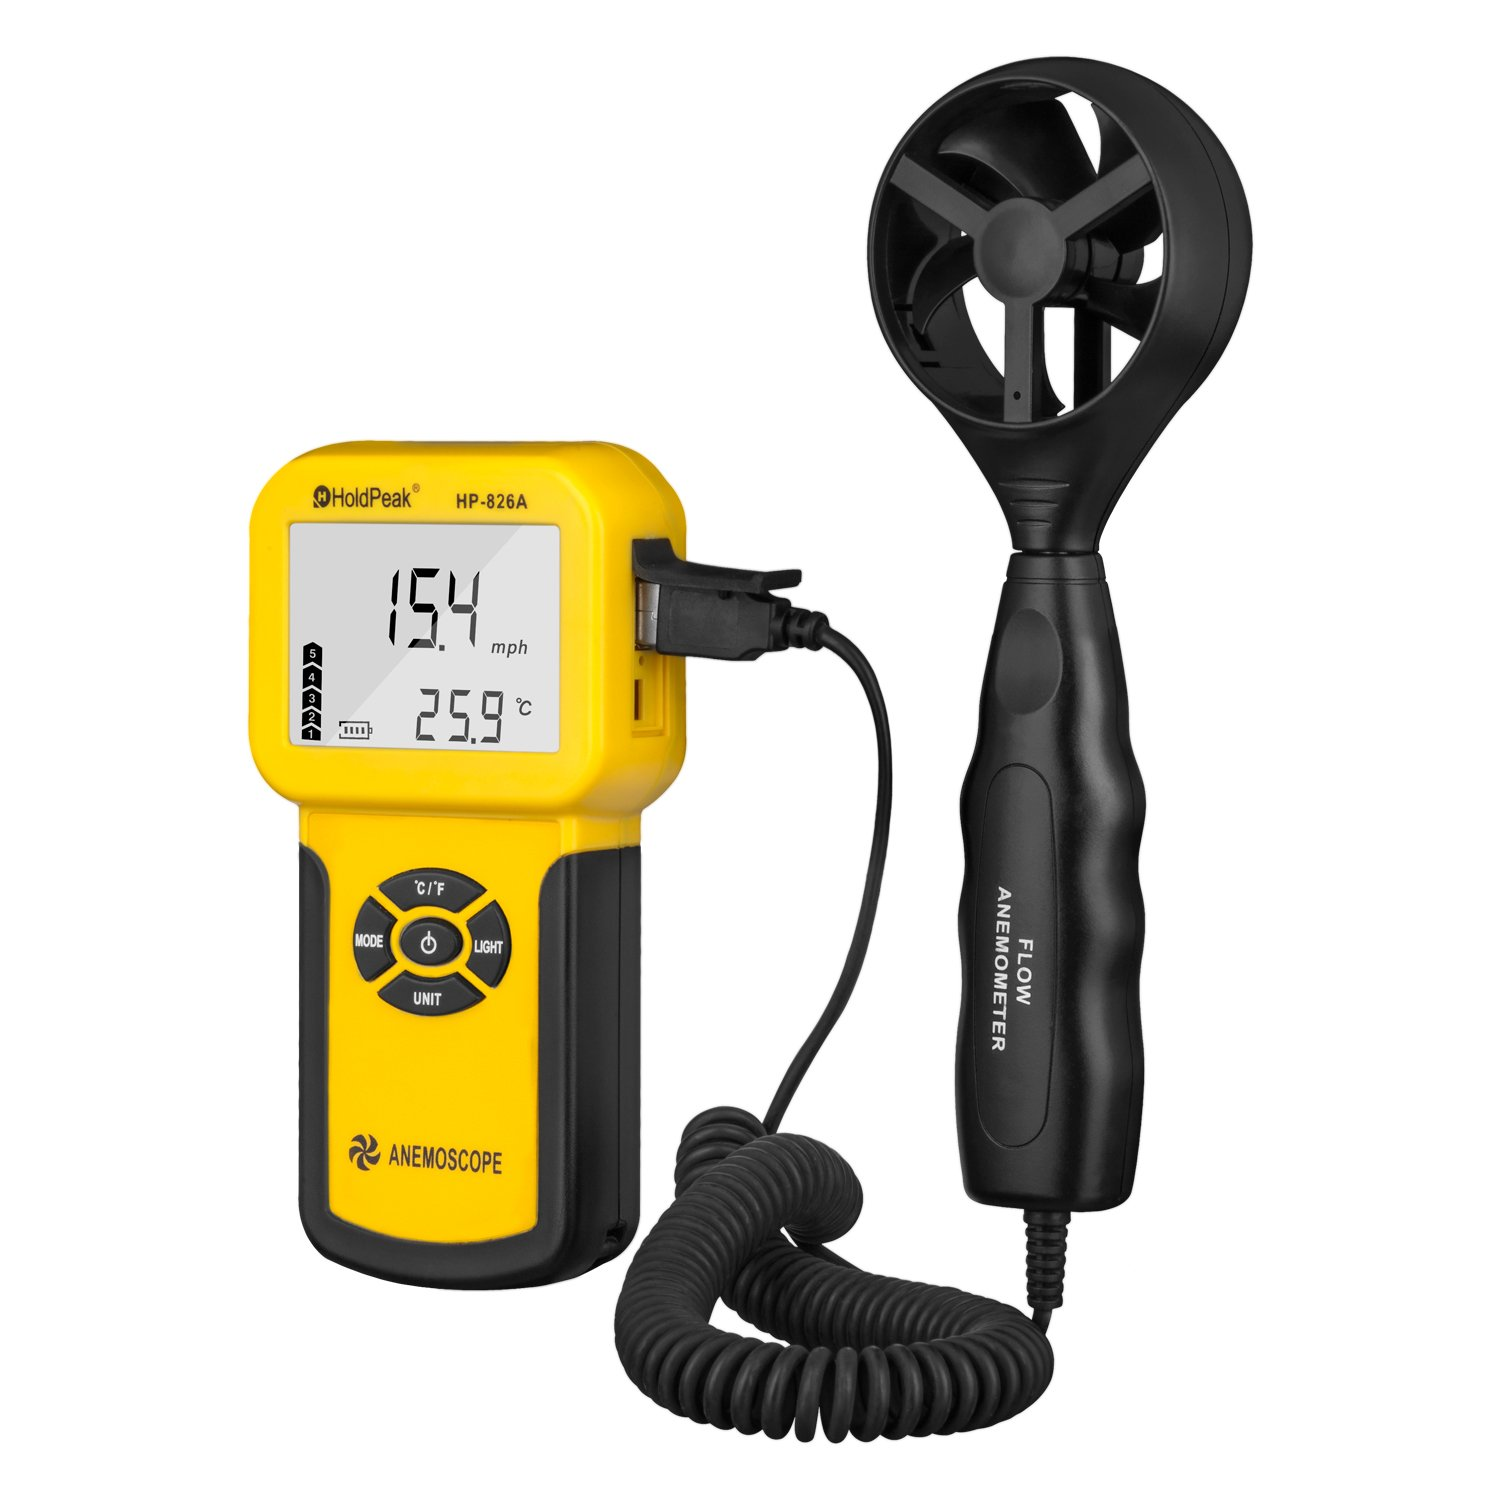
\includegraphics[
        width=0.5\textwidth,
        height=0.45\textwidth]
    {../Data/holdpeak.jpg}
    \caption{Picture of HoldPeak 822B}
    \label{fig:holdpeak}
\end{figure}

\subsubsection{Data Destruction}
\label{sec:analysis:erroranalysis:datadestruction}
The worst error introduced into this study is the loss of the wind speed data of Club Field and South Field from the HolePeak. Since a Rasberry Pi was used to record the data coming from the HoldPeak 
instrument sine HoldPeak officially only provide a windows-based application and it is unrealistic to use a laptop computer to collect data because its battery will not last for 24 hours, we determined 
that we are not going to measure the wind speed data during rainy days because Rasberry Pi is not water-proof. However, failure to check the newest weather report on 5/21/2019 resulted in Rasberry Pi's 
exposure in rain for an extended period of time - about 1 hour and caused the main circuit board of the Rasberry Pi to short out, burning out the Micro-SD card that was holding the wind speed data. Because 
of the ill-preparedeness that CL and Aaron had toward accidents like this, we did not previously backup the data on Rasberry Pi onto another computer. Therefore, every recorded wind speed data for Club Field 
and South Field were destroyed and lost, leaving us with only the data from the AQM65 on top of Dickinson Auditorium.


\clearpage
\bibliography{mybibfile.bib}    

\end{document}

%%However, both sites have a potential commono problem when considering their influence on school operations for their proximity to areas of student activity - club field and south field host wide array of atheletic activities during spring and fall trimester, and club field is right next to the hockey rink and Hoerle Hall.
%%Considering the area needed on the ground level, as well as the noise generated by the spinning blade, both sites, with the establishment of a wind farm, might generate negative influence on students daily activities. The distance from the wind farm to areas of student activities, i.e. Hockey Rink, Club Field itself, Hoerle Hall, and South Field itself will be approximated during the study and their influence analyzed.
%%But since those two sites are the only possible and viable locations due to the first and the second requirement, we will still take these two locations into consideration.

%%lub field is next to the Kent School main campus as well as the Mount Algos. By constructing a wind farm on club field, it will alter the landscape of the Mount Algos looking from the Kent campus and the landscape of Kent campus looking from the Mount Algos.
%%A wind farm on south field will change the landscape of the Housatonic river bank.